\subsection{Comparación entre una función logarítmica y una potencia}
\label{sec:act2-2}

\begin{enunciado}
Demuestre por definición que
\[
  n \log_2 n \in \Oh{n^{3/2}}.
\]
Debe encontrar constantes explícitas $c > 0$ y $n_0$ tales que
\[
  n \log_2 n \le c\, n^{3/2}
\]
para todo $n \ge n_0$. Como parte de la demostración, justifique una desigualdad
suficiente entre $\log_2 n$ y $\sqrt{n}$ a partir de algún $n_0$. No utilice límites ni
L'Hôpital.
\end{enunciado}

Según la definición vista en clases, $n \log_2 n \in \Oh{n^{3/2}}$ si existen una
constante $c > 0$ y un $n_0 \in \N$ tales que $0 \le n \log_2 n \le c\, n^{3/2}$ para
todo $n \ge n_0$. La primera desigualdad se cumple para todo $n \ge 1$, porque
$\log_2 n \ge 0$.

Como $n^{3/2} = n \cdot \sqrt{n}$ y $n > 0$, podemos dividir ambos lados por $n$:
\[
  n \log_2 n \le c\, n \sqrt{n} \iff \log_2 n \le c \sqrt{n}.
\]
Entonces basta mostrar que $\log_2 n \le \sqrt{n}$ desde algún $n_0$, y tomar $c = 1$.

Esta desigualdad no se cumple para todo $n$, como muestra la
figura~\ref{fig:act2-log-vs-raiz}.
\begin{figure}[H]
  \centering
  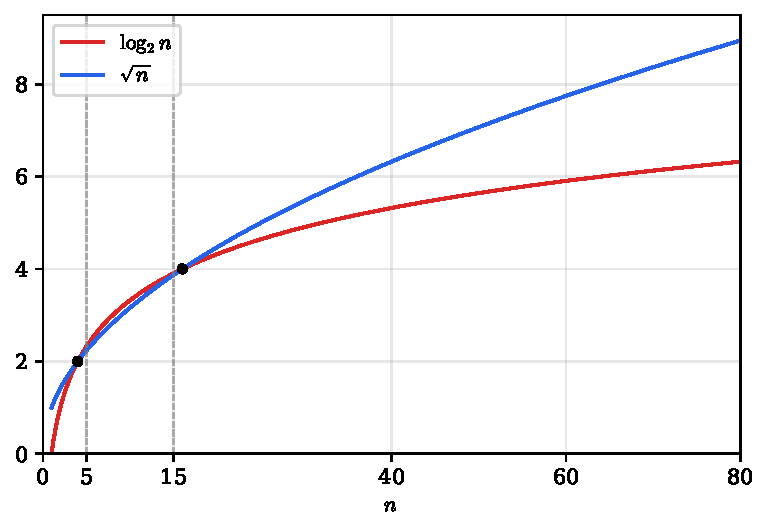
\includegraphics[width=0.75\linewidth]{act2_log_vs_raiz.pdf}
  \caption{$\log_2 n$ y $\sqrt{n}$ para $1 \le n \le 80$. Los puntos marcan los cruces
  en $n = 4$ y $n = 16$, y las líneas rayadas marcan $n = 5$ y $n = 15$, el primer y el
  último entero donde $\log_2 n > \sqrt{n}$. Generada con
  \texttt{scripts/act2\_log\_vs\_raiz.py}.}
  \label{fig:act2-log-vs-raiz}
\end{figure}
Las dos curvas se cruzan en $n = 4$, donde ambas valen $2$, y en $n = 16$, donde ambas
valen $4$. Entre esos dos puntos el logaritmo queda por encima de la raíz, así que la
desigualdad falla para todos los enteros entre $5$ y $15$. Por eso hay que elegir un $n_0$
a partir del cual la desigualdad se cumpla siempre.

Para comparar $\log_2 n$ con $\sqrt{n}$, ubicamos $n$
entre dos potencias de 2 seguidas. Sea $k = \floor{\log_2 n}$, de modo que
\[
  2^k \le n < 2^{k+1}.
\]
De ahí salen dos desigualdades. Aplicando logaritmo a $n < 2^{k+1}$, queda
$\log_2 n < k + 1$. Y sacando raíz a $2^k \le n$, queda $\sqrt{2^k} \le \sqrt{n}$.
Entonces, si mostramos que
\[
  k + 1 \le \sqrt{2^k},
\]
tendremos $\log_2 n < k + 1 \le \sqrt{2^k} \le \sqrt{n}$, que es lo que buscamos. Como
ambos lados son positivos, $k + 1 \le \sqrt{2^k}$ es lo mismo que $(k + 1)^2 \le 2^k$.

Ahora demostramos por inducción que $(k+1)^2 \le 2^k$ para todo $k \ge 6$.
\begin{itemize}
  \item \textbf{Caso base, $k = 6$:} $(6 + 1)^2 = 49 \le 64 = 2^6$.
  \item \textbf{Paso inductivo:} suponemos que $(k+1)^2 \le 2^k$ para algún $k \ge 6$
        (hipótesis de inducción) y mostramos que la desigualdad también vale para $k + 1$.
        Al reemplazar $k$ por $k + 1$, el lado izquierdo $(k+1)^2$ pasa a ser $(k+2)^2$ y
        el lado derecho $2^k$ pasa a ser $2^{k+1}$, así que hay que probar
        \[
          (k+2)^2 \le 2^{k+1}.
        \]
        Escribimos $k + 2$ como $(k+1) + 1$ y desarrollamos el cuadrado de un binomio,
        $(a + 1)^2 = a^2 + 2a + 1$, con $a = k + 1$:
        \[
          (k+2)^2 = \big((k+1) + 1\big)^2 = (k+1)^2 + 2(k+1) + 1 = (k+1)^2 + 2k + 3.
        \]
        El primer término, $(k+1)^2$, es el que aparece en la hipótesis. Ahora acotamos
        el resto, $2k + 3$, por ese mismo término. Restando,
        \[
          (k+1)^2 - (2k+3) = k^2 + 2k + 1 - 2k - 3 = k^2 - 2,
        \]
        y $k^2 - 2 > 0$ para $k \ge 6$ (de hecho, para todo $k \ge 2$). Luego
        $2k + 3 < (k+1)^2$, y reemplazando en la expresión de $(k+2)^2$:
        \[
          (k+2)^2 = (k+1)^2 + (2k + 3) \le (k+1)^2 + (k+1)^2 = 2\,(k+1)^2.
        \]
        Por la hipótesis de inducción, $(k+1)^2 \le 2^k$, y multiplicando por 2 queda
        $2\,(k+1)^2 \le 2 \cdot 2^k = 2^{k+1}$. Juntando las dos desigualdades:
        \[
          (k+2)^2 \le 2\,(k+1)^2 \le 2^{k+1},
        \]
        que es lo que había que probar.
\end{itemize}
Por lo tanto, $(k+1)^2 \le 2^k$ para todo $k \ge 6$. El caso $k = 5$ no sirve, porque
$36 > 32$.

Con esto, si $n \ge 64 = 2^6$, entonces $k = \floor{\log_2 n} \ge 6$, y por
lo anterior
\[
  \log_2 n \le \sqrt{n} \qquad \text{para todo } n \ge 64.
\]
Multiplicando ambos lados por $n$:
\[
  n \log_2 n \le n \sqrt{n} = 1 \cdot n^{3/2}.
\]
Luego, $c = 1$ y $n_0 = 64$. Por lo tanto, $n \log_2 n \in \Oh{n^{3/2}}$.

